\documentclass[12pt]{article}
\usepackage{setspace}
\setstretch{1}
\usepackage{amsmath,amssymb, amsthm}
\usepackage{graphicx}
\usepackage{bm}
\usepackage[hang, flushmargin]{footmisc}
\usepackage[colorlinks=true]{hyperref}
\usepackage[nameinlink]{cleveref}
\usepackage{footnotebackref}
\usepackage{url}
\usepackage{listings}
\usepackage[most]{tcolorbox}
\usepackage{inconsolata}
\usepackage[papersize={8.5in,11in}, margin=1in]{geometry}
\usepackage{float}
\usepackage{caption}
\usepackage{esint}
\usepackage{url}
\usepackage{enumitem}
\usepackage{subfig}
\usepackage{wasysym}
\newcommand{\inlinecode}{\texttt}
\usepackage{etoolbox}
\usepackage{algorithm}
% \usepackage{algorithmic}
\usepackage[noend]{algpseudocode}
\usepackage{tikz}
\usetikzlibrary{matrix,positioning,arrows.meta,arrows}
\patchcmd{\thebibliography}{\section*{\refname}}{}{}{}

\makeatletter
\renewcommand{\@seccntformat}[1]{}
\makeatother


\begin{document}



\title{\textbf{EECS 325: Assignment 1}}

\author{Shaochen (Henry) ZHONG, \inlinecode{sxz517} }
\date{Due and submitted on 02/06/2020 \\ EECS 325, Dr. WANG}
\maketitle

\section{Question 1}

\subsection{1.a.}

\begin{gather}
    \text{Transmission Delay} = \frac{\text{Average Packet Length}}{\text{Transmission Rate}} = \frac{125\cdot 8 \  \text{bits}}{10^8 \ \text{bits/s}} = 10^{-5} \ \text{sec}
\end{gather}

\subsection{1.b.}

\begin{gather}
    \text{Traffic Intensity} =  \frac{80 \cdot 1000 \cdot 125 \cdot 8 \  \text{bits}}{10^8 \ \text{bits}} = 0.8 \\
    \Longrightarrow \text{Average Queue Length} = \frac{\text{Traffic Intensity}}{\text{$1 - $Traffic Intensity}} = \frac{0.8}{1-0.8} = 4 \ \text{Packets}
\end{gather}

\subsection{1.c.}

% \begin{gather}
%     \text{Average Waiting Time} = \frac{\text{Total Wait Time for All Packets}}{\text{Number of Queued Packets}} \nonumber \\
%     \Longrightarrow \ = \frac{0 + 10^{-5} + 2 \cdot 10^{-5}  + 3 \cdot 10^{-5}}{4} = 1.5 \cdot 10^{-5} \ \text{sec}
% \end{gather}

\begin{gather}
    \text{Average Waiting Time} = \text{Average Queue Length} \cdot \text{Transmission Delay}  = 4 \cdot 10^{-5} \ \text{sec}
\end{gather}


\section{Question 2}

\subsection{2.a.}

\begin{gather}
    \text{Length of Packets} = \frac{10^7 \ \text{bytes}}{1000 \
    \text{bytes}} \cdot (1000 + 60) = 1.06 \cdot 10^7 \ \text{bytes}\\
    d_{\text{trans}} = \frac{L}{R} = \frac{1.06 \cdot 10^7 \cdot 8\ \text{bits}}{4 \cdot 10^6 \ \text{bps}} = 21.2 \ \text{sec}
\end{gather}

\subsection{2.b.}

\begin{gather}
    \frac{\text{Goodput}}{R} = \frac{\text{Payload}}{\text{Length of Packets}} \\
    \Longrightarrow \text{Goodput} = \frac{10 \ \text{mb}}{106 \ \text{mb}} \cdot 4 \ \text{mbps} = 3.77 \ \text{mbps}
\end{gather}


\section{Question 3}

\subsection{3.a.}

\begin{gather}
    d_{\text{prop}} = \frac{\text{Distance Traveled}}{\text{Propagation Speed}} = \frac{2 \cdot 750 \cdot 1000 \ \text{m}}{3 \cdot 10^{8} \ \text{m/s}} = 0.005 \ \text{s}
\end{gather}

\subsection{3.b.}

\begin{gather}
    d_{\text{trans}} = \frac{L}{R} = \frac{1250 \cdot 8\ \text{bits}}{100 \cdot 10^6 \ \text{bps}} = 0.0001 \ \text{sec}\\
    \text{Average Throughput} = \frac{L}{d_{\text{trans}} + \ 2(d_{\text{prop}})} = \frac{1250 \cdot 8\ \text{bits}}{0.0002 + 2(0.005)} = 990,099 \ \text{bps}
\end{gather}

\subsection{3.c.}

\begin{gather}
    \text{Average Throughput} = \frac{x}{ d_{\text{trans}} + \ 2(d_{\text{prop}})} = \frac{x \ \text{bits}}{0.0001 + 2(0.005)} = 100 \cdot 10^6 \ \text{bps} \nonumber\\
    \Longrightarrow x = 1,010,000 \ \text{bits}
\end{gather}

\section{Question 4}


\subsection{4.a.}

\begin{gather}
    d_{\text{trans}} = \frac{1500 \cdot 8\ \text{mb}}{1 \ \text{Mbps}} + \frac{1500 \cdot 8\ \text{mb}}{0.5 \ \text{Mbps}} + \frac{1500 \cdot 8\ \text{mb}}{1 \ \text{Mbps}} + \frac{1500 \cdot 8\ \text{mb}}{2 \ \text{Mbps}} \\
    = (12 + 24 + 12 + 6) \ \text{ms} = 54 \ \text{ms} \nonumber\\
    \Longrightarrow \text{Total Time}  = d_{\text{trans}} + d_{\text{prop}} = 54 + (2 + 20 + 30 + 2) = 108 \ \text{ms}
\end{gather}


\subsection{4.b.}

\begin{gather}
    d_{\text{total}} = (3 \cdot d_{\text{trans}_{1}} + d_{\text{prop}}) + (2 \cdot d_{\text{trans}_{2}} + d_{\text{prop}}) + (d_{\text{trans}_{3}} + d_{\text{prop}}) + (d_{\text{trans}_{4}} + d_{\text{prop}}) \\
    = (3 \cdot 12 + 2) + (2 \cdot 24 + 20) + (12 + 30) + (6 + 2) = 156 \ \text{ms} \nonumber
\end{gather}

\subsection{4.c.}

Packet 12, 14, 16, 18, 20 will be dropped according to [\figurename{ \ref{figure_1}}].

\begin{figure}
    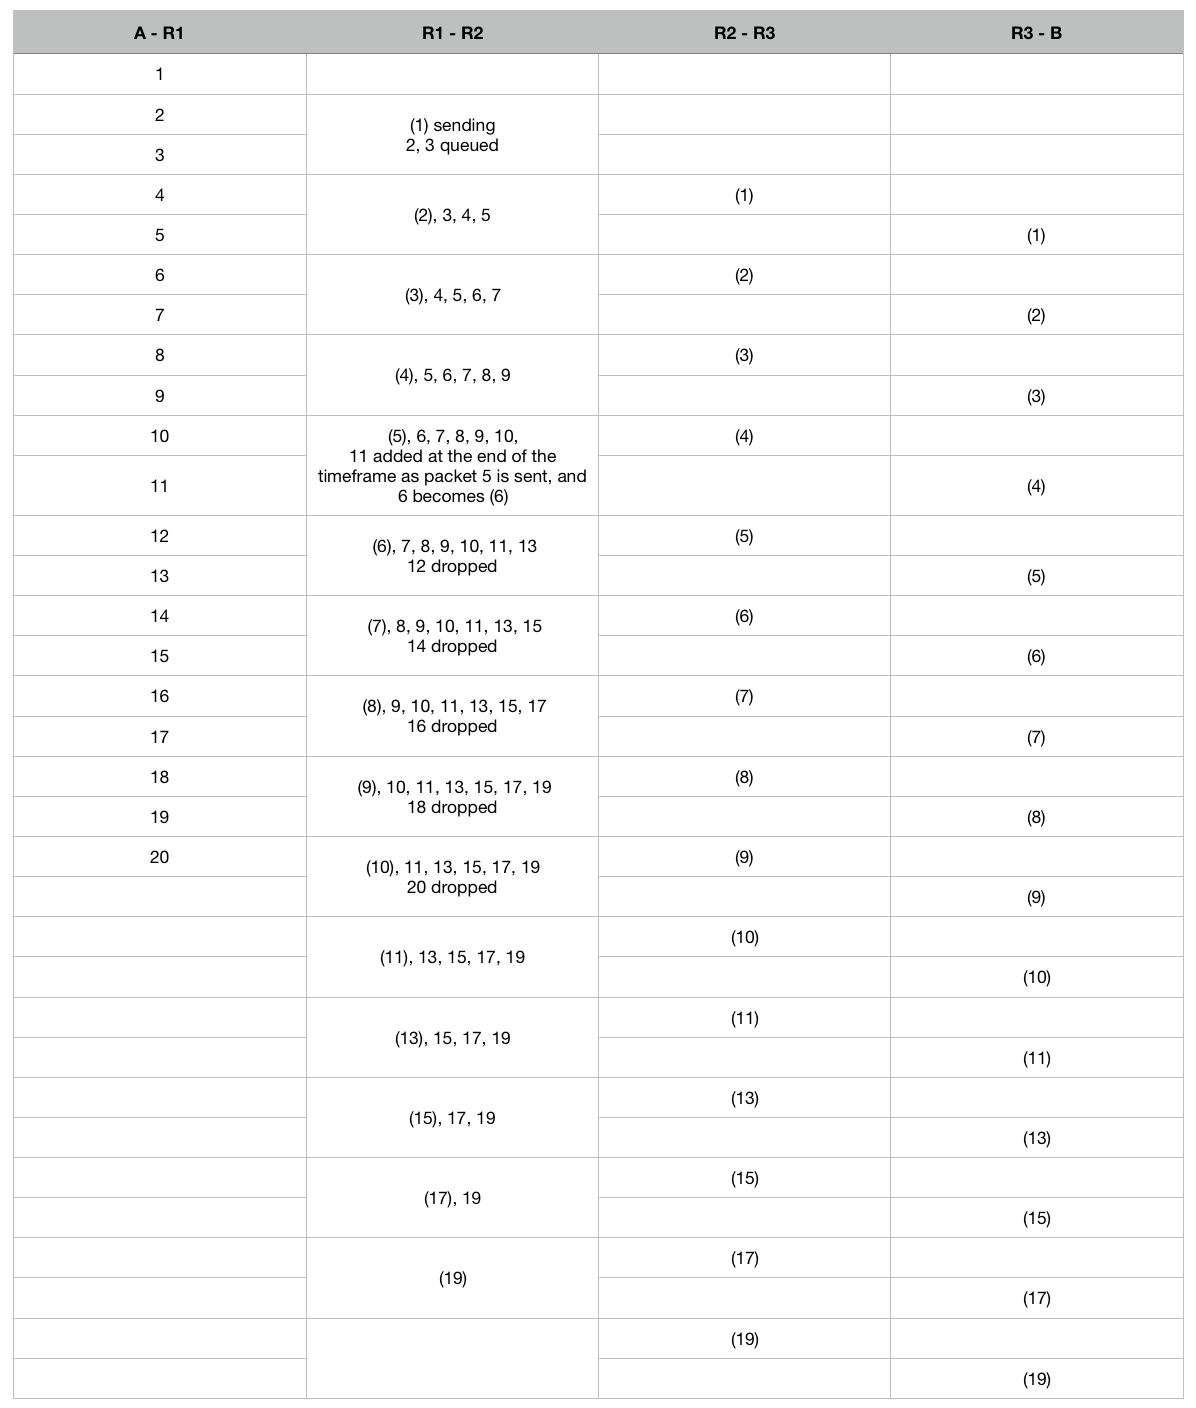
\includegraphics[width = .745\textwidth]{figure_1.png}
    \caption{Packets Queue Visualization from A to B}
    \label{figure_1}
\end{figure}

\newpage

\subsection{4.d.}
\subsubsection{4.d.a}
The worst-case end-to-end delay from $A$ to $B$ will happen if a packet is considered to be the 6th packet in the queue of $R1$, as it is added due to one packet of $R1$ has just been sent. By such case such packet must wait through $5 \cdot d_{\text{trans}_{2}}$ plus a standard $d_{\text{total}}$ calculated in \textit{Question 4}.

\begin{gather}
    d_{\text{max}_{AB}} = 5 \cdot d_{\text{trans}_{2}} + d_{\text{total}} \\
    = 5 \cdot 24 + 108 = 228 \ \text{ms} \nonumber
\end{gather}

\subsubsection{4.d.b}
he worst-case end-to-end delay from $B$ to $A$ will happen if a packet is considered to be the 6th packet in the queue of $R3$, as it is added due to one packet of $R3$ has just been sent, then it encounters the scenario of \textbf{Section 4.d.a} By such case such packet must wait through $5 \cdot d_{\text{trans}_{3}}$ (there will be 5 packets queued since $d_{\text{trans}_{4}} = 2 \cdot d_{\text{trans}_{3}}$, an identical relationship as $d_{\text{trans}_{1}}$ and $d_{\text{trans}_{2}})$, then $5 \cdot d_{\text{trans}_{2}}$, plus a standard $d_{\text{total}}$ calculated in \textit{Question 4}.



\begin{gather}
    d_{\text{max}_{BA}} = 5 \cdot d_{\text{trans}_{3}} + 5 \cdot d_{\text{trans}_{2}}  + d_{\text{total}} \\
    = 5 \cdot 12 + 5 \cdot 24+ 108 = 288 \ \text{ms} \nonumber
\end{gather}

% \section{References}
%
% \nocite{*}
% \raggedright
% \bibliography{references.bib}
% \bibliographystyle{plain}


\end{document}